\chapter{(A) Introduzione alla libreria e aspetti implementativi}
\section{Econofisica e \textit{option pricing}} \label{sec:introduction_econophysic_option_pricing}
In ambito finanziario si definisce \textit{titolo derivato} un contratto il cui valore dipende da un prodotto finanziario più fondamentale, detto \textit{bene sottostante} o semplicemente \textit{sottostante}. Obiettivo di questa relazione è lo studio di un tipo particolare di titolo derivato, ovvero le \textit{opzioni europee}, definibili, nella loro forma più elementare, come contratti che garantiscono il diritto di compravendita del sottostante in una data futura (detta \textit{data di maturità}) a un prezzo fissato (detto \textit{prezzo di esercizio}). A seconda delle caratteristiche del tipo di opzione prescelto, ciò frutterà al suo acquirente un rendimento $P$ detto \textit{pay-off}.

Un primo esempio di contratto derivato analizzato in questa trattazione è il contratto a termine \textit{forward}, con un \textit{pay-off} definito da
\begin{equation}
    P_f = S(T),
    \label{eq:forward_pay-off}
\end{equation}
dove $T$ è la data di maturità e $S(t)$ il prezzo del sottostante al tempo $t$. Questo tipo di contratto, a differenza delle opzioni, obbliga entrambe le parti coinvolte a onorarlo.

Altra tipologia di derivato studiata è quella delle opzioni \textit{plain vanilla}, definite come \textit{call} o \textit{put} a seconda che assicurino il diritto di comprare o vendere il sottostante. Nel caso delle \textit{plain vanilla call} il \textit{pay-off} è dato da
\begin{equation}
    P_{pvc} = {\left[S(T)-E\right]}^+,
    \label{eq:pvc_pay-off}
\end{equation}
mentre nelle \textit{plain vanilla put} è dato da
\begin{equation}
    P_{pvp} = {\left[E-S(T)\right]}^+,
    \label{eq:pvp_pay-off}
\end{equation}
dove $E$ è il prezzo di esercizio e $+$ indica che consideriamo solo la parte positiva dell'espressione.

Un esempio di opzione più sofisticata, che sarà anche l'oggetto di studio principale nel nostro progetto, è costituito dall'opzione di tipo \textit{performance corridor}, il cui \textit{pay-off} è dato da
\begin{equation}
    P_{pc} = N\left[ \frac{1}{m} \sum_{i=0}^{m-1}{P_i} - K \right]^+,
    \label{eq:performancecorridor_pay-off}
\end{equation}
dove
\begin{equation}
    P_i = \begin{cases}
    1, & \text{se} \,\,\left| \frac{1}{\sqrt{\Delta t}} \log{\frac{S(t_{i+1})}{S(t_i)}} \right| < B \sigma;\\
    0, & \text{altrimenti}.
  \end{cases}
    \label{eq:performancecorridor_barrier}
\end{equation}

Questo è un caso di opzione \textit{path-dependent}, in quanto il \textit{pay-off} è funzione della percentuale di volte in cui il rendimento logaritmico del sottostante in modulo tra due date di rilevazione rimane confinato all'interno di una barriera la cui altezza è parametrizzata da $B$. In questo contesto la variabile $K$ rappresenta una sorta di <<prezzo di esercizio>> in percentuale, mentre $N$ è il nozionale a cui la percentuale risultante dal calcolo del \textit{pay-off} viene applicata.

In virtù dell'\textit{assioma di non arbitraggio}, il quale afferma che non è possibile realizzare un guadagno certo a un rendimento superiore al tasso di interesse privo di rischio, il prezzo equo delle opzioni è stabilito sulla base del \textit{pay-off} delle opzioni stesse. Essendo quest'ultimo dipendente dall'andamento del prezzo del sottostante tra la data odierna e la data di maturità, il problema del \textit{pricing} delle opzioni è legato a doppio filo alla necessità di modellizzare l'evoluzione del valore del sottostante nel tempo.

Uno dei modelli più diffusi per questo scopo è quello del \textit{moto browniano geometrico}, basato sull'assunto che il prezzo $S(t)$ del sottostante segua un processo lognormale con tasso d'interesse privo di rischio $r$ e volatilità $\sigma$ fissati, ovvero
\begin{equation}
    \frac{dS}{S} = r dt + \sigma \sqrt{dt} w,
    \label{eq:lognormal}
\end{equation}
dove $w$ è una variabile casuale estratta da una distribuzione normale di media nulla e varianza unitaria. Dividendo l'intervallo $[0,T]$ in $m$ date di rilevazione $t_i$ di distanza $\Delta t$, si calcola il prezzo $S(t_{i+1})$ in funzione del prezzo attuale $S(t_i)$ secondo la formula
\begin{equation}
    S(t_{i+1}) = S(t_i) \exp{\left[\left(r- \frac{\sigma^2}{2}\right)\Delta t + \sigma \sqrt{\Delta t} w\right]}.
    \label{eq:exactprice}
\end{equation}

Nell'approssimazione di un intervallo $\Delta t$ sufficientemente ridotto\footnote{Per un approfondimento sui limiti di applicabilità di questa approssimazione, consultare la Sezione \ref{sec:limits}.}, l'equazione \eqref{eq:lognormal} può essere risolta con una tecnica semplificata arrivando alla formula alternativa
\begin{equation}
    S(t_{i+1}) \approx S(t_i) \left(1 + r \Delta t + \sigma \sqrt{\Delta t} w\right).
    \label{eq:eulerprice}
\end{equation}

Nel corso della relazione faremo riferimento alla soluzione \eqref{eq:exactprice} come \textit{schema esatto} e alla \eqref{eq:eulerprice} come \textit{schema di Eulero}. Iterando questi schemi sull'intero lasso di tempo d'elezione, è possibile effettuare \textit{simulazioni} dell'evoluzione del prezzo del sottostante e conseguentemente stabilire il \textit{pay-off} medio di un'opzione alla data di maturità.

Ciò non è tuttavia sufficiente a determinare il prezzo equo dell'opzione, poiché il valore di un determinato capitale in data odierna $t=0$ non corrisponde al valore del medesimo capitale in una data futura $T>0$; ciò avviene perché la definizione stessa di tasso di interesse \textit{privo di rischio} implica che il denaro nel tempo è in grado di generare con probabilità certa ulteriore denaro\footnote{Nel corso dei nostri studi abbiamo sempre assunto un tasso di interesse privo di rischio $r$ positivo.}. Per tale ragione è necessario \textit{attualizzare} il \textit{pay-off} attraverso la formula
\begin{equation}
    P_0 = P_T e^{-rT}.
    \label{actualization}
\end{equation}


\section{Panoramica del codice} \label{sec:code_generics}
Le caratteristiche del problema dell'\textit{option pricing} lo rendono particolarmente adatto a essere affrontato con una metodologia di tipo \textit{single instruction, multiple data} (SIMD), un'architettura in cui un insieme di processori eseguono il medesimo algoritmo su flussi di dati differenti; un codice progettato secondo questa filosofia sarà infatti in grado di eseguire un elevato numero di simulazioni del prezzo del sottostante in parallelo, ottimizzando i tempi di esecuzione.

La piattaforma di sviluppo CUDA progettata dalla Nvidia Corporation si presta in modo particolare a questo tipo di architettura in quanto le GPU su cui il codice viene eseguito sono caratterizzate da un elevato numero di \textit{core} in grado di eseguire operazioni elementari. La libreria oggetto di questa relazione è stata quindi da noi sviluppata in linguaggio CUDA/C++ per trarre vantaggio da tali peculiarità; per una discussione più approfondita circa i vantaggi di questo approccio rispetto al più semplice CUDA/C, riferirsi al Capitolo \ref{cap:cudacpp}.

\begin{figure}
    \centering
    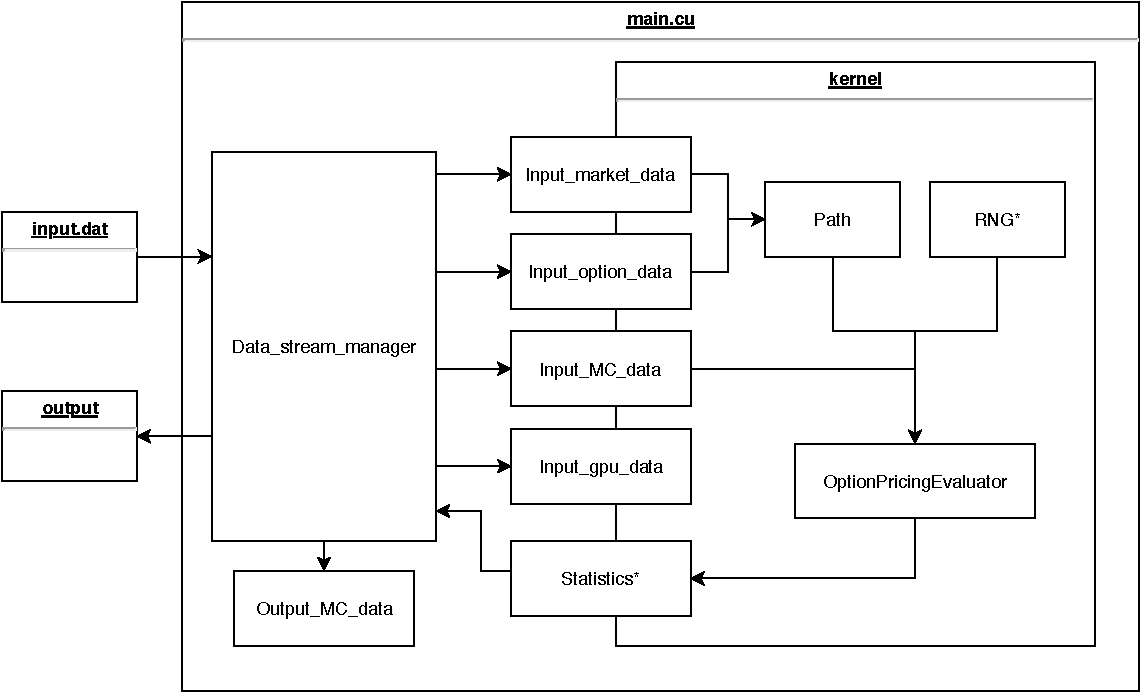
\includegraphics[scale=0.8]{graphs/RecapMainCuDiagram.pdf}
    \caption[Diagramma del funzionamento dell'eseguibile principale della libreria.]{Diagramma riassuntivo del funzionamento dell'eseguibile principale della libreria; gli asterischi in \texttt{\textcolor{blue}{RNG*}} e \texttt{\textcolor{blue}{Statistics*}} indicano un puntatore a una classe derivata nel primo caso e un vettore allocato dinamicamente nel secondo.}
    \label{fig:diagram}
\end{figure}

In Figura \ref{fig:diagram} è rappresentato un diagramma riassuntivo del funzionamento dell'eseguibile primario della libreria, orientato all'\textit{option pricing}. Il listato integrale del codice appositamente commentato è riportato in Appendice \ref{app:allcode}; a seguire ne saranno illustrati i punti principali.

Al primo livello di complessità, classi, strutture e funzioni di supporto della libreria da noi progettata sono suddivise in tre macrocategorie:

\begin{itemize}
    \item \textbf{strutture di \textit{input}}: strutture elementari per la memorizzazione dei dati riguardanti le opzioni (\codeword{Input_option_data}), il mercato (\codeword{Input_market_data}), la GPU (\codeword{Input_gpu_data}) e le simulazioni Monte Carlo (\codeword{Input_MC_data});
    \item \textbf{struttura di \textit{output}}: struttura singola (\codeword{Output_MC_data}) che raccoglie i risultati delle simulazioni Monte Carlo;
    \item \textbf{librerie principali}: classi C++ che gestiscono e manipolano i dati nelle simulazioni, discusse di seguito.
\end{itemize}

La prima libreria principale per ordine logico è la classe astratta \codeword{RNG} che gestisce la generazione di numeri pseudocasuali. Nel codice sono implementate due tipologie di generatori concreti: un generatore Tausworthe puro basato su un registro a scorrimento a retroazione lineare (\codeword{RNG_Tausworthe}) e un generatore combinato basato su tre generatori Tausworthe e un generatore lineare congruenziale (\codeword{RNG_CombinedGenerator}).

A partire dai numeri generati da un puntatore \codeword{RNG*}, la classe \codeword{Path} gestisce i singoli passi del processo lognormale esatto \eqref{eq:exactprice} e della versione approssimata di Eulero \eqref{eq:eulerprice}, calcolando i \textit{pay-off} $P_i$ delle opzioni. Questi ultimi sono processati dalla classe \codeword{Statistics}, che ne calcola la media $\braket{P_i}$ e l'errore
\begin{equation}
    \epsilon_\text{MC} = \sqrt{\frac{\braket{P_i^2} - \braket{P_i}^2}{N}}
    \label{eq:mcerror}
\end{equation}

Infine la classe \codeword{Data_stream_manager} gestisce l'interazione dell'utente con il flusso di dati in entrata e in uscita, interpretando i dati indicati nel file \verb|input.dat|, scrivendo i risultati di \textit{output} in un oggetto \codeword{Output_MC_data} e stampando a schermo le informazioni sulle simulazioni effettuate.

L'interazione tra le varie componenti del codice è organizzata dal metodo  \codeword{OptionPricing Evaluator(...)}, programmato nelle sue varianti \codeword{__global__}, \codeword{__host__} e \codeword{__device__ __host__} secondo il paradigma \textit{host-device} approfondito in Sezione \ref{sec:cpugpu}. La funzione principale \codeword{main()}, secondo i desideri dell'utente, esegue tale algoritmo su CPU o GPU invocando due funzioni ausiliarie \codeword{CPUOptionPricingMonteCarloAlgorithm(...)} e \codeword{GPUOptionPricingMonteCarloAlgorithm(...)}.

\begin{table}[t]
\small
\centering
\begin{tabular}{|l||l|l|}
\hline
\textbf{GPU} & \textit{Tesla P100-PCIE-12GB} & \textit{Tesla C2075} \\
\hline \hline
\textbf{CUDA Driver version} & 10.1 & 9.1 \\ \hline
\textbf{CUDA Runtime version} & 10.1 & 8.0 \\ \hline
\textbf{CUDA Capability version} & 6.0 & 2.0 \\ \hline
\textbf{Global memory} & 12 GB &  5 GB \\ \hline
\textbf{Maximum clock rate} & 1.33 GHz & 1.15 GHz \\ \hline
\textbf{Multiprocessors} & 56 & 14 \\ \hline
\textbf{CUDA Cores} & 3584 & 448 \\ \hline
\textbf{Constant memory} & 65 kB & 65 kB \\ \hline
\textbf{Shared memory per block} & 49 kB & 49 kB \\
\hline
\end{tabular}
\caption{Specifiche tecniche delle due schede grafiche in nostra dotazione per le simulazioni.}
\label{tab:hardware}
\end{table}

\section{Specifiche hardware} \label{sec:hardware}
La maggior parte delle simulazioni da cui sono stati ottenuti i risultati illustrati nella presente relazione è stata effettuata su una scheda grafica di modello \verb|Tesla P100-PCIE-12GB|. Occasionalmente, e in modo significativo negli studi sul tempo di esecuzione in Sezione \ref{sec:comptime}, abbiamo fatto uso di una meno performante \verb|Tesla C2075|. In Tabella \ref{tab:hardware} sono riportate le specifiche hardware delle due GPU.